\section{Driving Factors of Network Congestion}\label{sec:factors}

With mobile devices becoming smarter, smaller, and ubiquitous, consumers are embracing the technology and driving up the demand for mobile data.  According to Cisco's VNI \cite{CiscoVNImobile}, in 2012, global mobile data traffic grew more than 70 percent year over year, to 855 petabytes a month. The growth rate varied by regions, with 44\% growth in Western Europe, and about 101\% in the Middle East and Africa and a 95\% growth rate in Asia Pacific. This section identifies some of the key factors that are expected to drive this growth in demand for mobile data (ref. Figure \ref{fig:driving_factors}).

\begin{figure}[h]
\centering
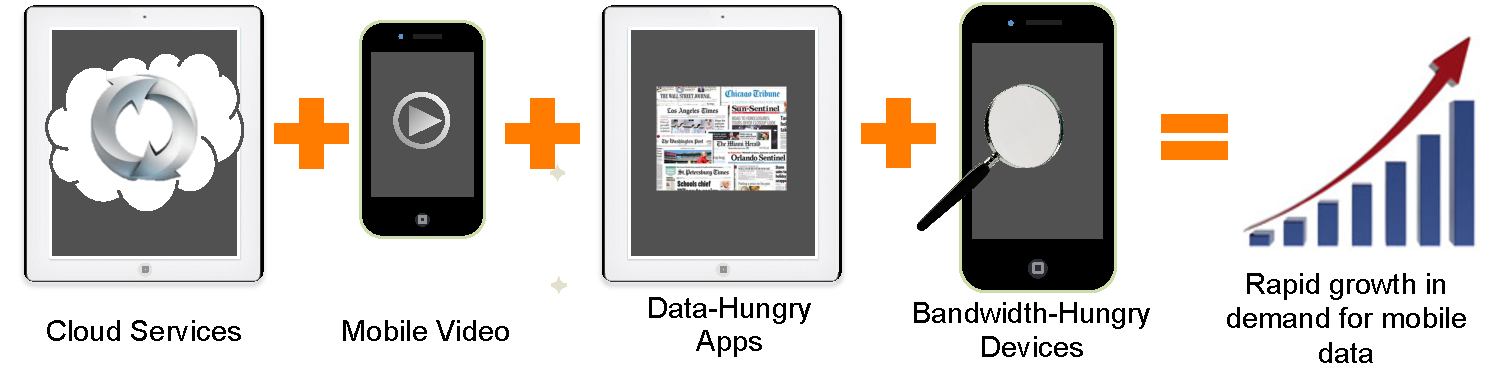
\includegraphics[width = 0.9\textwidth]{Figures/Driving_factors.pdf}
\vspace{-0.1in}
\caption{Factors driving the demand for mobile data.}
\label{fig:driving_factors}
\vspace{-0.05in}
\end{figure}

{\bf\emph{Cloud Services and M2M Applications:}}
Cloud-based services that synchronize data across multiple mobile devices, such as iCloud, Dropbox, and Amazon�s Cloud Drive, can be a significant factor in traffic growth for ISPs \cite{icloud}. Similarly, machine-to-machine (M2M) applications that generate data intermittently (e.g., sensors and actuators, smart meters) or continuously (e.g., video surveillance) often load the network with large signaling overhead \cite{BellLabs}.  However, these traffic types also have some intrinsic time elasticities that create opportunities for intelligently shifting them to low-congestion times through pricing incentives. 

{\bf\emph{Mobile Videos:}}
Video has also been a major contributor to mobile data traffic growth, accounting for 51 percent of global mobile data traffic at the end of 2012. It is expected to account for 66 percent of global mobile data traffic by 2017 \cite{CiscoVNImobile}. A study by Gartner \cite{Gartner2012} states that the worldwide mobile video market had 429 million mobile video users in 2011, projected to grow exponentially to 2.4 billion users by 2016. Smartphones and tablet sales will contribute 440 million new mobile video users during the forecast period. The report also forecasts that the worldwide share of mobile video connections on 3G/4G will increase from 18\% in 2011 to 43\% in 2015 \cite{Goog-mobile}. These growth rates are being further fueled by mobile video content delivery via mobile-optimized websites and video advertisements.

{\bf\emph{Capacity-Hungry Applications:}}
The popularity of handheld devices has led to rapid growth in the development of other bandwidth-hungry applications for social networking, music, personalized online magazines, etc. in addition to file downloads and video streaming. Virgin Media Business reports that the average smartphone software uses 10.7 MB per hour, with the highest-usage app, Tap Zoo, consuming up to 115 MB/hour. In the current ecosystem, app developers do not have enough incentives to account for network conditions, and consequently many smartphone apps are not optimized for bandwidth consumption.

{\bf\emph{Bandwidth-Hungry Devices:}}
The widespread adoption of handheld devices, equipped with powerful processors, high-resolution cameras, and larger displays, has made it convenient for users to stream high-quality videos and exchange large volumes of data.  Data from laptops with 3G dongles and netbooks with wireless high-speed data access contributes the most to wireless network congestion \cite{BellLabs}.  As for smartphones, Cisco projects that the average monthly data usage will rise from 150 MB in 2011 to 2.6 GB in 2016 \cite{CiscoVNImobile}.  New features like Siri on the iPhone 4S, which has doubled Apple users' data consumption, are driving this growth \cite{siri}.

The key takeaways from the above discussion of the various factors contributing to network congestion are:
\begin{itemize}
\item Different types of applications and services have different levels of time elasticity of demand (e.g., cloud backup versus financial applications).
\item There is a great variance in the rate of growth of different types of applications (e.g., demand for mobile videos is growing fast).
\item Different applications consume bandwidth at different rates and have a large variance in QoE requirements (e.g., many apps are not optimized for bandwidth while some well-designed apps can adapt to available network QoS). 
\item There is a growing variance in the bandwidth requirements of different smart devices (e.g., iPad versus iPhone versus feature phones).
\end{itemize}
These factors contribute to the need for smarter data plans that can account for the variances across users' QoE needs, time elasticity of demand, application traffic characteristics and their willingness to pay for the service.

%These developments have led ISPs to view pricing as their ultimate congestion management tool, paving the way for the adoption of Smart Data Pricing (SDP) measures, such as time-dependent and usage-based pricing.
Before delving deeper into SDP's promise in addressing congestion issues \cite{SDPForum}, in the next section we first explore how these trends are impacting the various stakeholders of the network ecosystem, i.e., network operators, consumers, app developers, and content providers.